\section{Teste da Aplicação}

\subsection{Testes Unitários}

\par Os testes unitários foram realizados sobre a classe \textit{Client.java}.
Na figura abaixo pode-se ver a classe criada para os testes.\newline
Nesta classe, criaram-se as seguintes variáveis globais:
\begin{itemize}
\item 2 pontos;
\item 1 cliente;
\item 1 owner;
\end{itemize}

\par Adicionalmente criaram-se variáveis do objeto Car e Rental para verificar a correção de alguns métodos da classe visada.

\begin{figure}[H]

  \centering

  \hbox{\hspace{-6em} 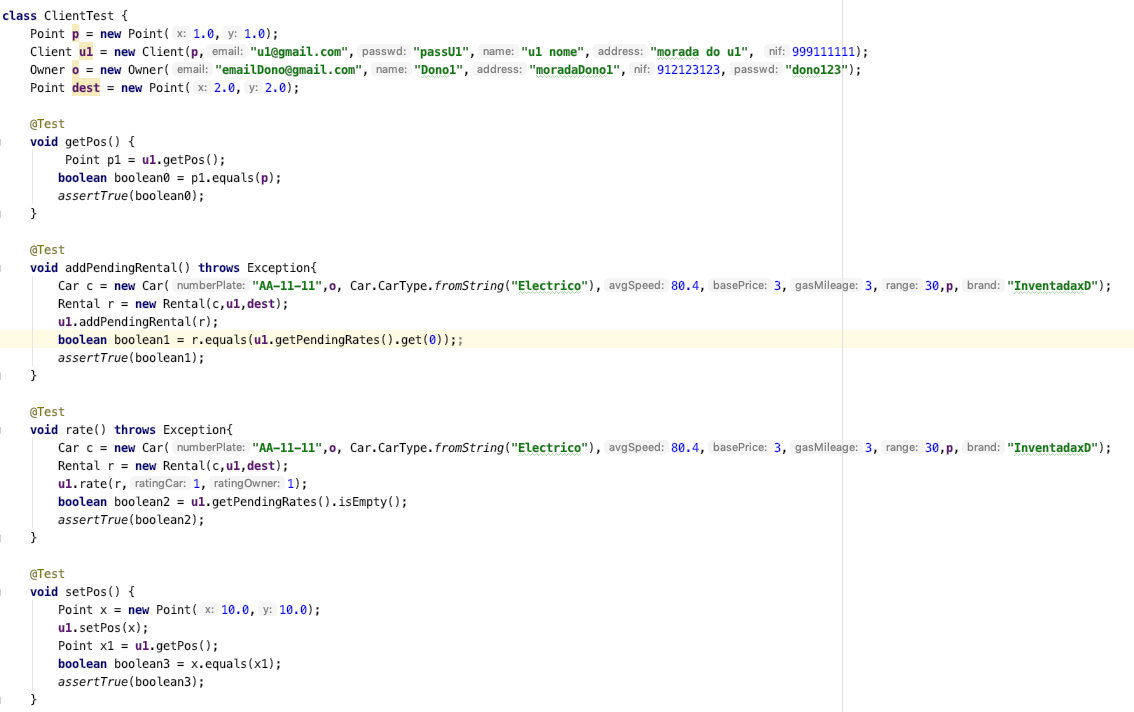
\includegraphics[scale = 0.40]{clientTest1.png}}

\end{figure}

\begin{figure}[H]

  \centering

  \hbox{\hspace{-8em} 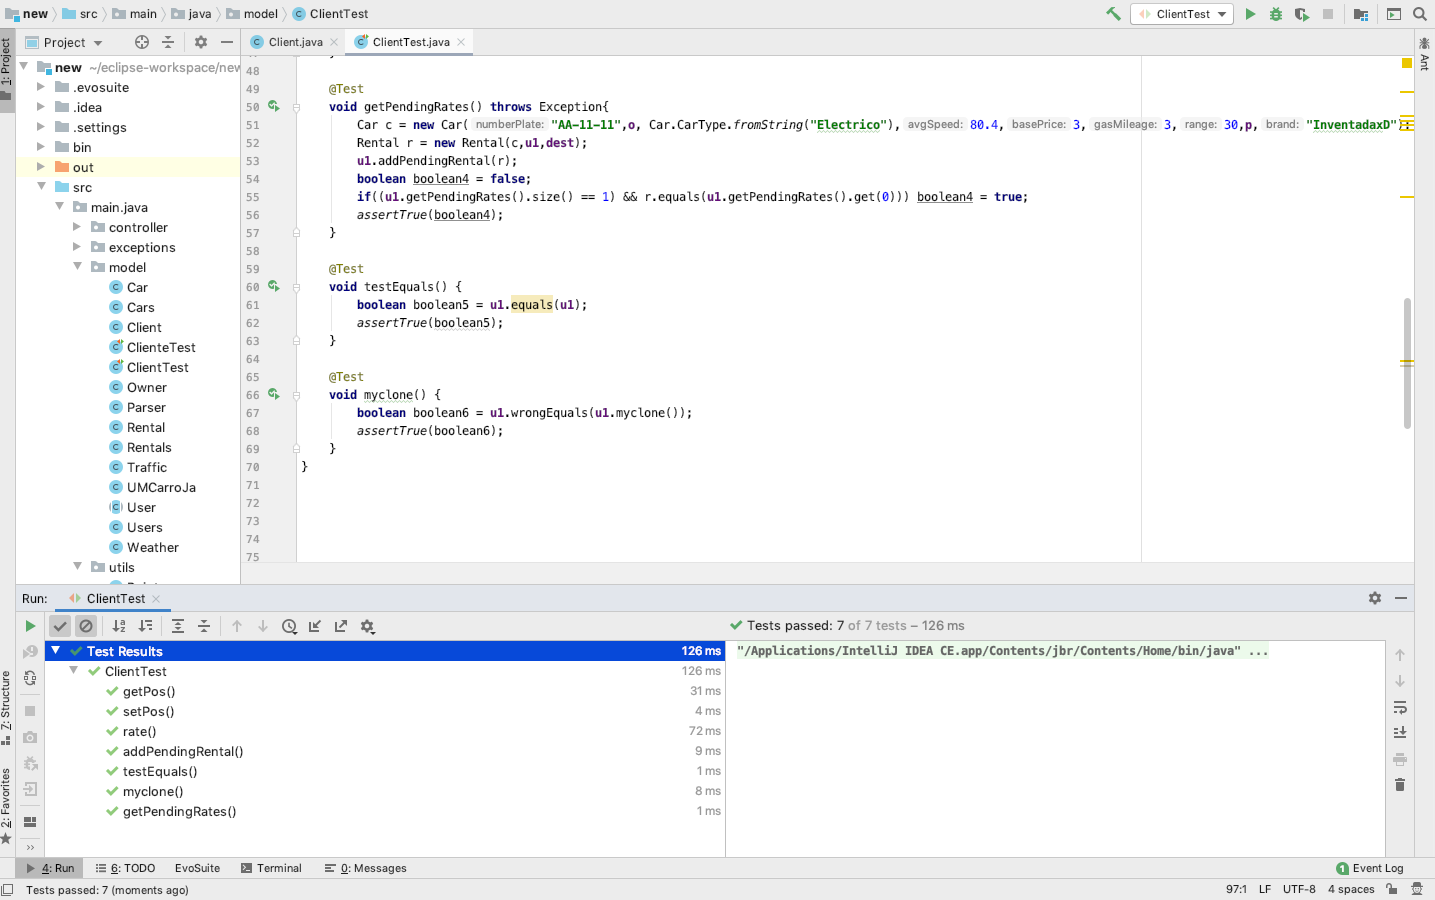
\includegraphics[scale = 0.35]{clientTestResults.png}}

  \caption {Classe ClientTest.java e resultado da sua aplicação}

  \label {fig30}

\end{figure}
\par Note-se que para testar a correção do método \textit{myclone()} foi criado um método extra na classe Cliente para verificar se os clientes partilhavam o mesmo apontador, esse método foi chamado \textit{wrongEquals()}.

\par Na figura seguinte podemos ver o código coberto por este ficheiro de testes.\newline

\begin{figure}[H]

  \centering

  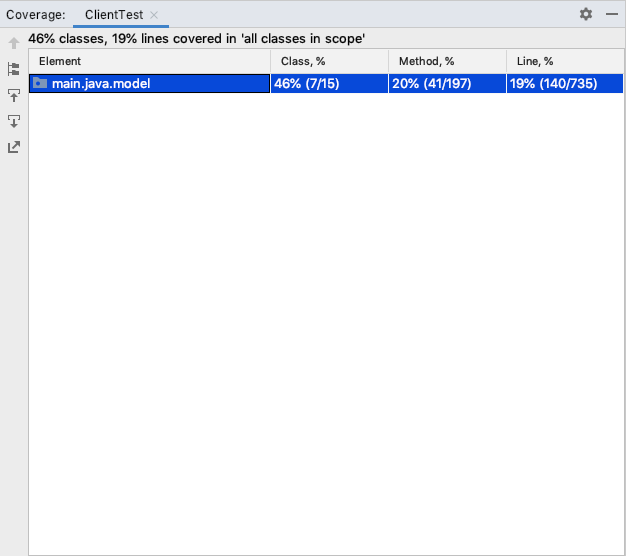
\includegraphics[scale = 0.45]{coverageClient.png}

  \caption {Cobertura da classe ClientTest.java sobre o package main.java.model}

  \label {fig31}

\end{figure}

\par \textit{Nota1:} Note-se que o facto do teste cobrir 46\% das classes do package main.java.model e 20\% dos métodos deve-se á necessidade, por parte da classe visada, de incluir objetos e recorrer a métodos de outras classes do mesmo package para ser completamente testada.\newline
\par \textit{Nota2:} Note-se que o teste de cobertura só abrange o package main.java.model. No entanto, a classe testada utiliza uma classe de nome \textit{Point.java} de outro package.

\subsection{Evosuite}

\subsubsection{Geração de testes}

\par Para compilar o Evosuite precisei de instalar um plugin chamado Choose Runtime no InteliJ. Este foi usado para escolher a versão do JDK 1.8.0\_231 como a versão a usar para correr o Evosuite. Após correr o Evosuite para gerar os teste o resultado mostra-se nas seguintes figuras.

\begin{figure}[H]

  \centering

  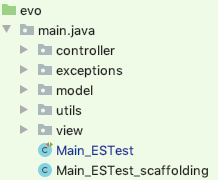
\includegraphics[scale = 0.45]{evoMain.png}

  \caption {Testes class Main}

  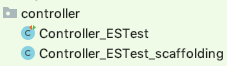
\includegraphics[scale = 0.45,trim = 0 0 0 -2cm]{evoController.png}

  \caption {Testes package Controller}

  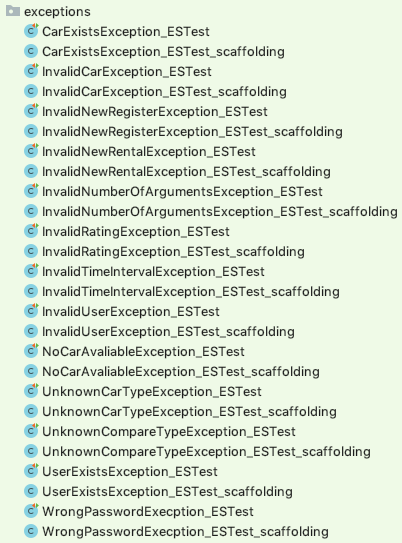
\includegraphics[scale = 0.45,trim = 0 0 0 -2cm]{evoExceptions.png}

  \caption {Testes do package exceptions}

  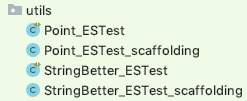
\includegraphics[scale = 0.45,trim = 0 0 0 -2cm]{evoUtils.png}

  \caption {Testes do package utils}
  \label {fig35}

\end{figure}  
\begin{figure}[H]

  \centering
  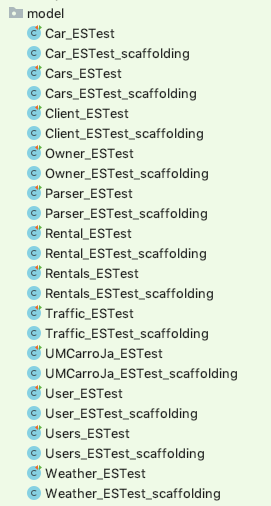
\includegraphics[scale = 0.45,trim = 0 0 0 -2cm]{evoModel.png}

  \caption {Testes do package model}

  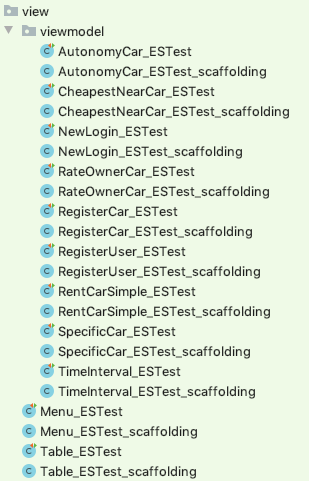
\includegraphics[scale = 0.45,trim = 0 0 0 -2cm]{evoView.png}

  \caption {Testes do package view}

  \label {fig36}

\end{figure}

\par Após o Evosuite gerar os ficheiros de teste, outro problema surgiu. Os ficheiros de teste não conheciam o jUnit apesar de este estar instalado. Para resolver este novo problema seguiram-se os seguintes passos:
\begin{itemize}
\item A primeira mudança para resolver este problema foi modificar a pasta onde os testes se encontravam para que fosse reconhecida como uma pasta de Sources root.
\item Em segundo lugar a pasta do Evosuite foi marcada como Test Sources Root.
\item Finalmente o ficheiro pom.xml foi alterado, adicionando como dependencia o Evosuite bem como adicionar nas propriedades o Evosuite.
\end{itemize}

\par Após a realização destes passos surgiu aquilo que parecia ser mais um problema. Nos ficheiros de teste gerados pelo Evosuite, este reconhece a class Main do projeto. No entanto, quando o Main é declarado este aparece a vermelho (como se estivesse errado) como se pode ver na figura abaixo.


\begin{figure}[H]

  \centering

  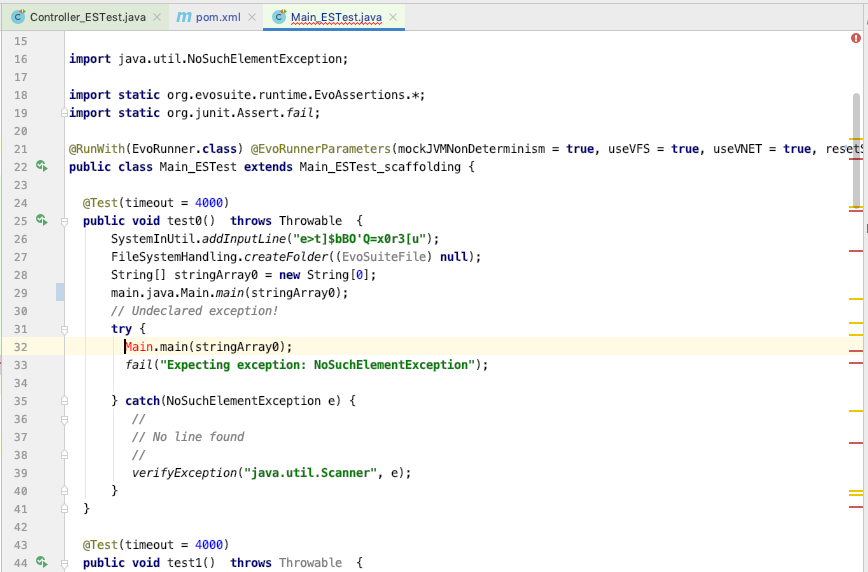
\includegraphics[scale = 0.45]{erroCertoMain_ESTest.png}

  \caption {Excerto do ficheiro Main\_ESTest}

  \label {fig38}

\end{figure}

\par no entanto o erro não se verifica uma vez que podemos correr o ficheiro sem problemas, o que nos leva a pensar que deve ser um erro de identificação do IDE.

\subsubsection{Verificação de classes utilizando os testes}

\par Após se ter confirmado a correta geração dos ficheiros de teste por parte do Evosuite procedeu-se a verificação das classes do nosso projeto com os mesmos.
\par A titulo de exemplo em seguida apresentam-se os resultados de alguns testes realizados sobre algumas das classes mais importantes do projeto em questão.

\begin{figure}[H]

  \centering

  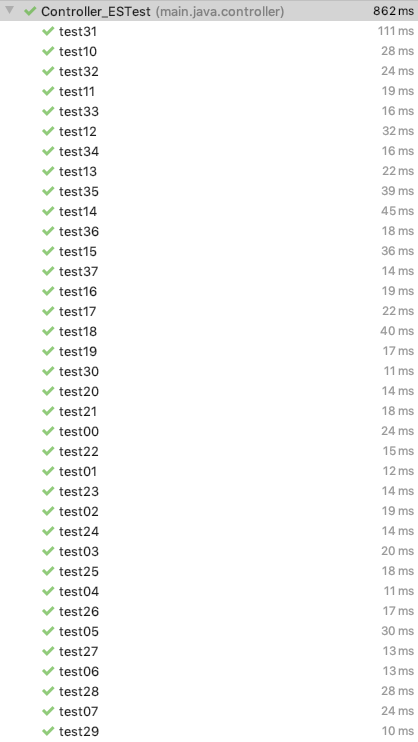
\includegraphics[scale = 0.45]{ControllerTests.png}
  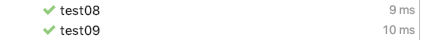
\includegraphics[scale = 0.45]{ControllerTests2.png}
  \caption {Resultados da execução do ficheiro Controller\_ESTest.java}

  \label {fig39}

\end{figure}
\begin{figure}[H]

  \centering

  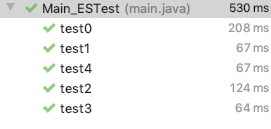
\includegraphics[scale = 0.45]{MainTests.png}

  \caption {Resultados da execução do ficheiro Main\_ESTest.java}

  \label {fig40}

\end{figure}
\begin{figure}[H]

  \centering

  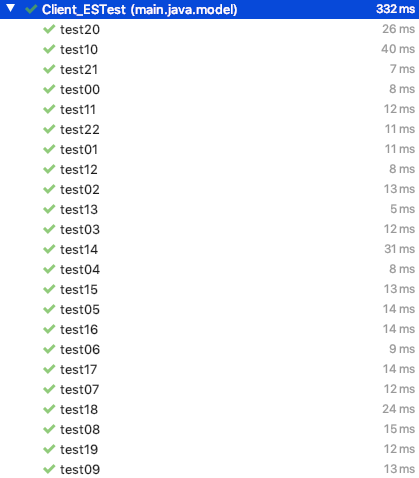
\includegraphics[scale = 0.45]{ClientTests.png}

  \caption {Resultados da execução do ficheiro Client\_ESTest.java}

  \label {fig41}

\end{figure}

\newpage
\subsection{Tests Coverage using JaCoCo}

\par Para realizar os testes com "coverage"  recorremos ao JaCoCo, como se pode ver na imagem abaixo.

\begin{figure}[H]

  \centering

  \hbox{\hspace{-8em}  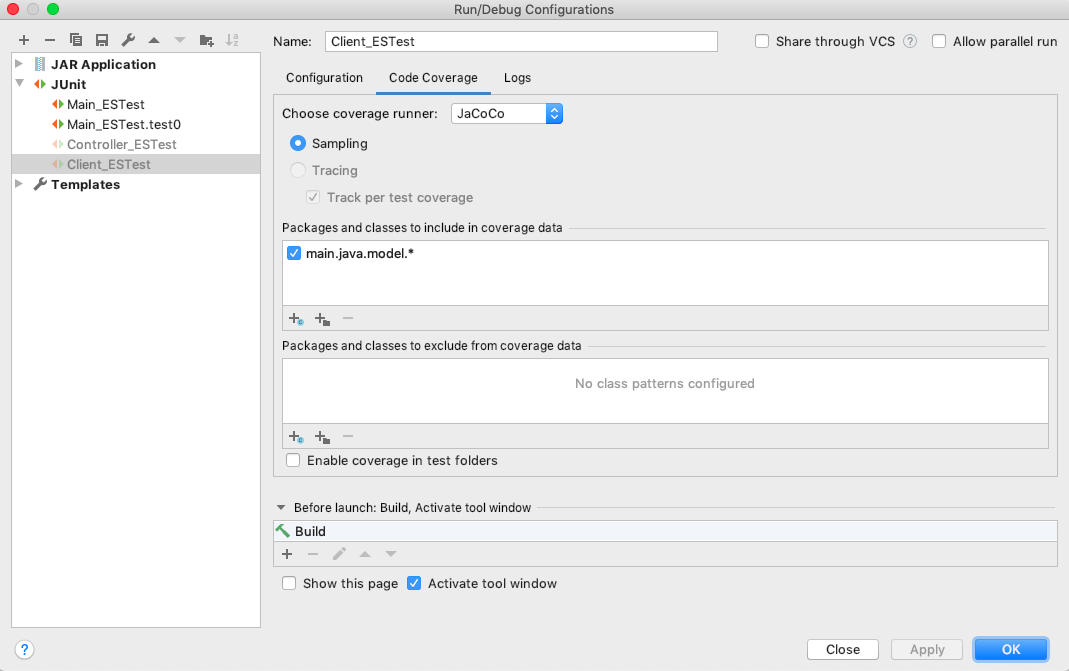
\includegraphics[scale = 0.45]{jacoco.png}}

  \caption {Configuração do Code Coverage para usar o  plugin JaCoCo}

  \label {fig42}

\end{figure}

\par Agora para correr os testes ao nosso programa basta-nos clicar no botão do canto superior direito assinalado na imagem seguinte para correr os testes com coverage.

\begin{figure}[H]

  \centering

  \hbox{\hspace{-10em} 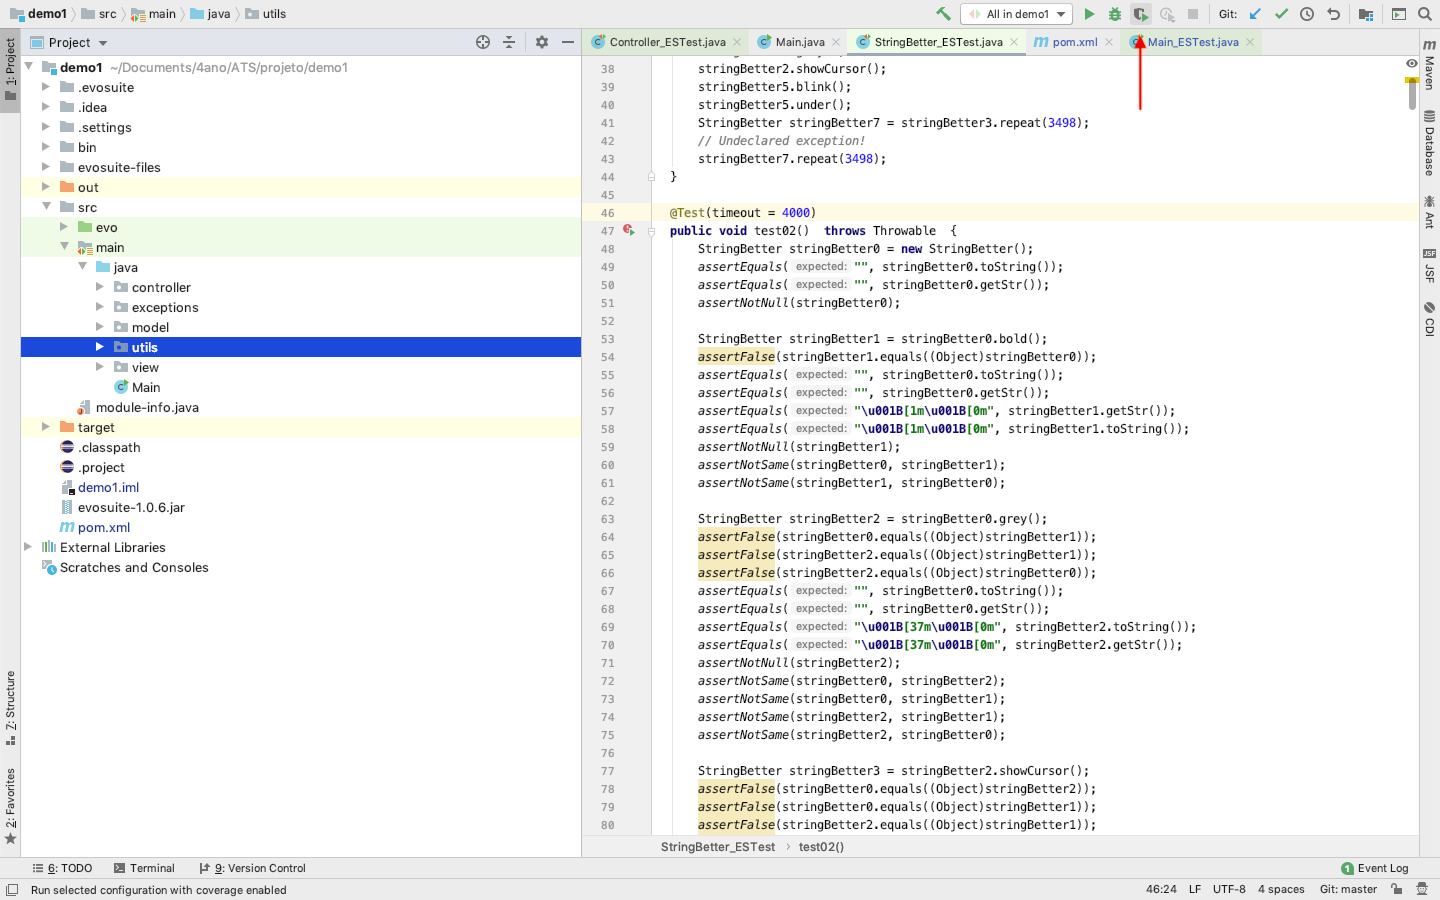
\includegraphics[scale = 0.35]{runCoverage.png}}

  \caption {Execução dos testes usando coverage com o plugin JaCoCo}

  \label {fig43}

\end{figure}

\par Por fim podemos ver os resultados do coverage das classes de cada package, em percentagem, na imagem abaixo.

\begin{figure}[H]

  \centering

  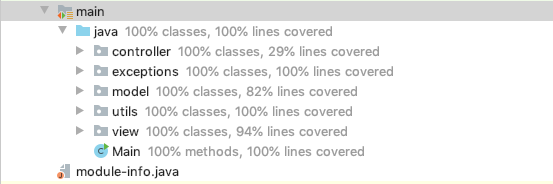
\includegraphics[scale = 0.45]{resultsCoverage.png}

  \caption {Resultados do coverage utilizando o plugin JaCoCo}

  \label {fig44}

\end{figure}

\par \textit{Nota3:} Note-se que um dos testes falhou na primeira execução, como se pode ver na seguinte imagem.

\begin{figure}[H]

  \centering

  \hbox{\hspace{-8em} 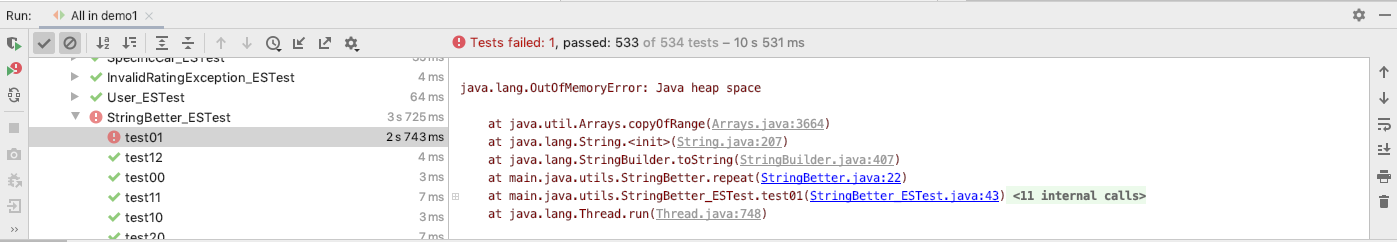
\includegraphics[scale = 0.45]{falhaTeste01.png}}

  \caption {Falha detetada no teste 01 referente a Java Heap Space}

  \label {fig44}

\end{figure}

\par Este problema acontece porque a Máquina virtual do Java tem um tamanho máximo de heap finito, isto leva a um erro como o que se pode verificar na imagem acima.










